% !TEX root SCHISADCJPOA JPFDÈOC KJ+ÒLDkc= ../Thesis.tex

\chapter{Primo approccio}
Il primo approccio divideva il problema in due parti. La prima è relativa alla previsine della qualità tramite tecniche 
di machine learning di immagini denoised. La seconda parte invece riguarda la fusione delle immagini.

\section{Previsione della qualità: dataset}



Come illustrato in Figura \ref{fig:MockReteNeurale}, il dataset impiegato è costituito da tre tipologie di 
immagini: clean, noisy e denoised. Queste immagini sono state realizzate tramite uno strumento ottico di un
satellite per poi essere sporcate con speckle artificiale e su cui infine è stato fatto denoising. Questa scelta è stata fatta
in quanto risulta difficile reperire un dataset contenente immagini SAR abbastanza grande da poter essere utlizzato per 
addestrare una rete neurale. Le immagini su cui viene fatto l'addestramento sono relative ad un singolo modello di despeckling ed ad 
un determinato look. Quest'ultimo è una metrica che indica l'intensità dello speckle artificiale, in quanto a più look.
corrispondono più catture di quella che è la realtà di interesse e quindi si ha una maggior precisione e uno speckle ridotto.
In fase di addestramento, le immagini noisy e denoised vengono concatenate in un unico tensore a due canali e utilizzate come 
input per la rete neurale. Le immagini clean, invece, assieme a quelle denoised, vengono impiegate per la 
generazione della mappa di qualità, che costituisce il riferimento necessario per 
il calcolo della funzione di perdita. Questo permette al modello di imparare a 
prevedere la qualità del denoising relative ad un dato modello di despeckling e ad una determinata intensità dello speckle. 
\begin{figure}[H]
    \centering
    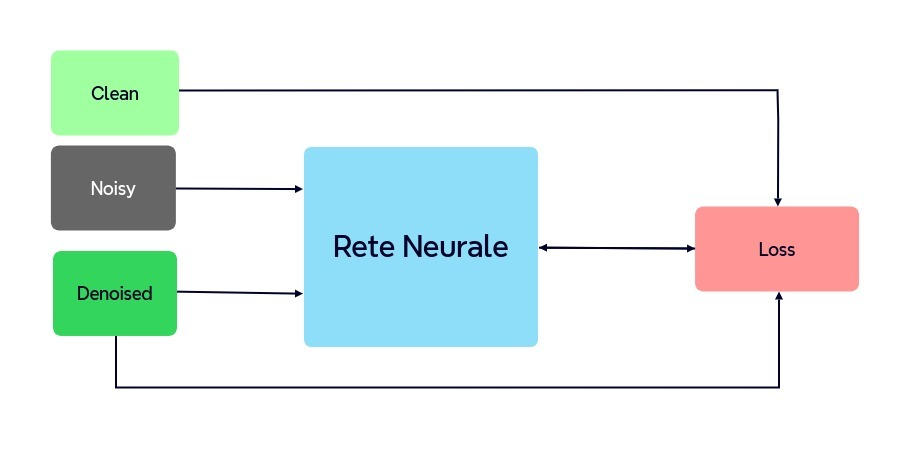
\includegraphics[width=0.8\textwidth]{utils/Architettura_rete_neurale.jpg}
    \caption{Mock della struttura logica per la previsione della qualità}
    \label{fig:MockReteNeurale}
\end{figure}

\section{Previsione della qualità: Architettura rete neurale}
Come Architettura della rete neurale è stata utilizzata la Unet. Questo perchè risulta particolarmente adatto per la 
generazione di una mappa di qualità che valuti l'affidabilità di un'immagine sottoposta a denoising. Il compito di 
questa rete è assegnare a ciascun pixel un valore continuo compreso nell'intervallo $[0,1]$ che ne rappresenti la 
qualità locale. Questo output per la sua natura richiede un'architettura in grado di produrre una mappa di densità 
della stessa risoluzione spaziale dell'input, preservando la localizzazione precise delle informazioni. 
L'architettura è composta da due bracci principali. Il braccio sinistro (encoder) opera una contrazione 
progressiva, applicando strati convoluzionali e di pooling per estrarre features astratte e gerarchiche 
dall'input. Questo processo permette alla rete di comprendere il contenuto semantico dell'immagine e la 
natura del rumore, apprendendo a riconoscere pattern complessi come texture, bordi e regioni omogenee. 
Il braccio destro (decoder) svolge il compito simmetrico di espansione, ricostruendo gradualmente la 
risoluzione spaziale attraverso operazioni di up-sampling e convoluzioni. È questa struttura ad "U" 
che permette di trasformare le feature astatte e globali apprese dall'encoder in una mappa 
dettagliata. L'elemento più innovativo dell'architettura U-Net è la presenza di connessioni skip che collegano i layer 
dell'encoder ai layer corrispondenti nel decoder. Questi collegamenti trasferiscono le mappe di feature 
ad alta risoluzione dalla fase di contrazione a quella di espansione. La loro presenza, è rilevante per la 
corretta generazione della mappa di qualità. Senza di esse, il decoder avrebbe perso l'informazione spaziale riguardante 
l'esatta localizzazione di dettagli critici come bordi sottili o piccole texture. Poiché sono proprio 
queste aree ad essere più suscettibili ad artefatti da oversmoothing o errata ricostruzione da parte degli 
algoritmi di denoising, le skip connections forniscono al decoder il contesto spaziale necessario per 
produrre una valutazione di qualità estremamente precisa e localizzata.Il modello deve superare la semplice stima 
di una differenza assoluta tra l'immagine denoised e un ground truth ideale. 
Deve invece sviluppare una percezione semantica dell'errore, ossia la capacità di valutare la gravità di una discrepanza 
in base al contesto visivo in cui appare. Un errore di grande entità in una regione uniforme (es. un cielo sereno) è 
percepibilmente molto più fastidioso di un errore di pari entità in una regione altamente texturizzata (es. del fogliame), 
dove può essere naturalmente mascherato. Analogamente, un piccolo errore di disallineamento su un bordo netto può essere molto 
visibile e quindi criticabile. L'encoder della U-Net, stratificando features da semplici a complesse, apprende automaticamente 
questa gerarchia di contenuti visivi. Il modello può dunque fondere la misura dell'errore con la comprensione del significato 
dell'area in cui esso si manifesta, producendo una mappa di qualità che pesa intelligentemente l'importanza visiva di ogni discrepanza.
\section{Fusione dei modelli}
La fusione delle immagini denoised $[I]$ prodotte tramite i rispettivi modelli di despeckling vengono fusi attraverso una media pesata sfuttando
le mappa di qualità $[M]$ come pesi per le singole immagini ovvero:
\begin{equation}
    \makebox[\textwidth][c]{%
      $\displaystyle
        \frac{\sum_{i=1}^{n} I_i M_i}{\sum_{i=1}^{n} M_i}
      $%
    }
\end{equation}
Non è una fusione "cieca" (es. una media semplice). È un processo che si 
comporta in modo diverso per ogni singolo pixel dell'immagine. Se il Modello A ha una qualità stimata 
molto alta in una regione e il Modello B molto bassa, la fusione privilegerà quasi esclusivamente 
il Modello A in quell'area. Mentre alcuni sono eccellenti nel preservare i bordi netti ma possono lasciare del rumore residuo nelle aree lisce, 
altri sono ottimi nell' eliminare il rumore dalle superfici lisce ma tendono a sfocare (oversmooth) i bordi e le texture.
La fusione pesata permette di prendere il meglio di ogni modello usando l'output dell'algoritmo migliore per una data 
caratteristica dell'immagine, scartando virtualmente i suoi contributi peggiori.
  
    